% Para experimentar, utilizamos una computadora con las siguientes características:

% \begin{itemize}
%  \item Procesador: 
%  \item RAM: 
% \end{itemize}

Al igual que en el problema \emph{Camiones Sospechosos}, la solución propuesta tiene la característica de que la complejidad temporal del algoritmo es dominada por la etapa de ordenamiento. Por esta razón, lo que mencionamos en la sección \ref{problema1-experimentacion} también vale en este caso: las instancias utilizadas para la medición se generaron de forma pseudo-aleatoria, limitando el análisis de los resultados al rendimiento de caso promedio. 

Adicionalmente, para corroborar que el ciclo posterior al ordenamiento incurre efectivamente en un costo a lo sumo lineal, continuamos la experimentación sobre instancias donde la lista de entrada se encuentra ordenada, eliminando la primer etapa. En este caso, dado que el ciclo no contiene ejecución condicional y siempre ejecuta exactamente la misma cantidad de instrucciones independientemente de la entrada, no se puede distinguir entre mejor y peor caso. Por esa razón, realizamos mediciones únicamente sobre instancias pseudo-aleatorias ordenadas según el coeficiente mencionado en \ref{problema2-desarrollo}.

\subsubsection{Incluyendo etapa de ordenamiento}

Medimos el tiempo de ejecución al resolver instancias de entre 1 y 10000 piezas, según las consideraciones de la sección \ref{consideraciones-mediciones}, permitiendo graficar el costo temporal de la implementación en función del tamaño de entrada $T(n)$. En la figura (\ref{fig:problema2-aleatoria-10000}) se observan los resultados obtenidos.

\begin{center}
  \begin{figure}[H]
    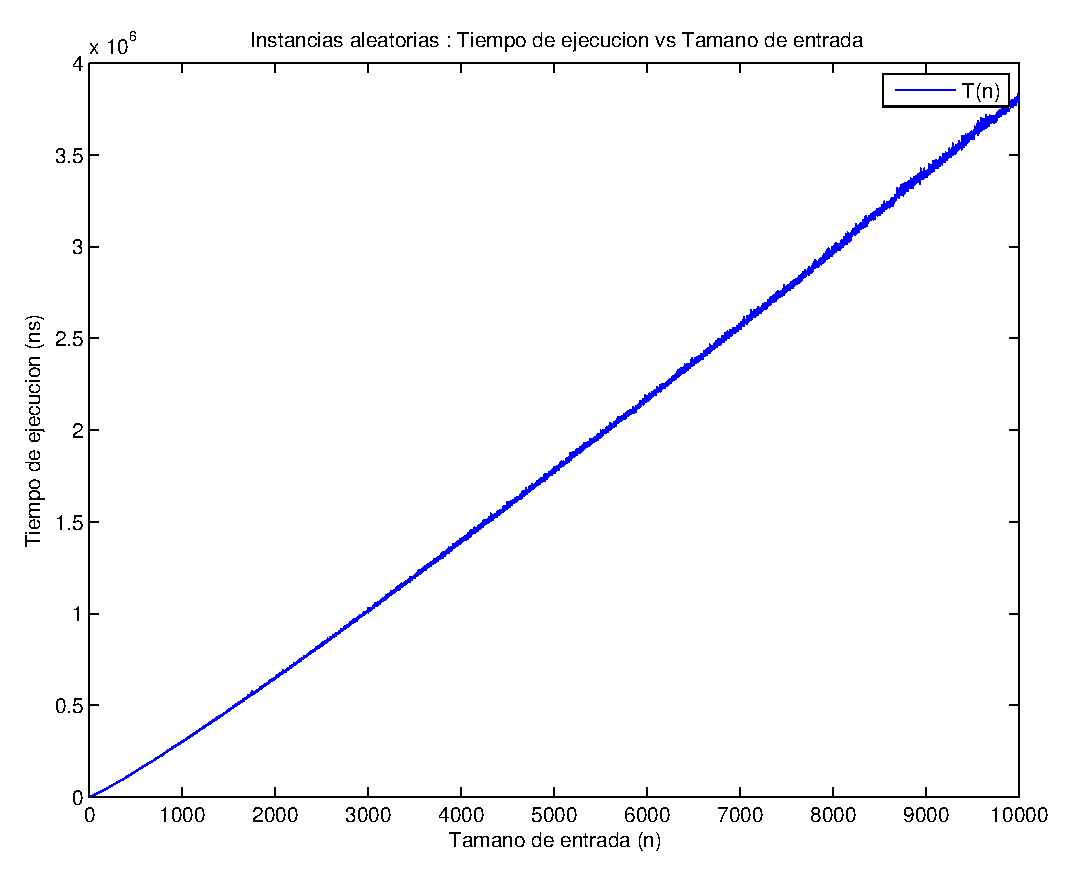
\includegraphics[width=0.5\linewidth]{problema2/graficos/problema2_aleatoria_10000.eps}
    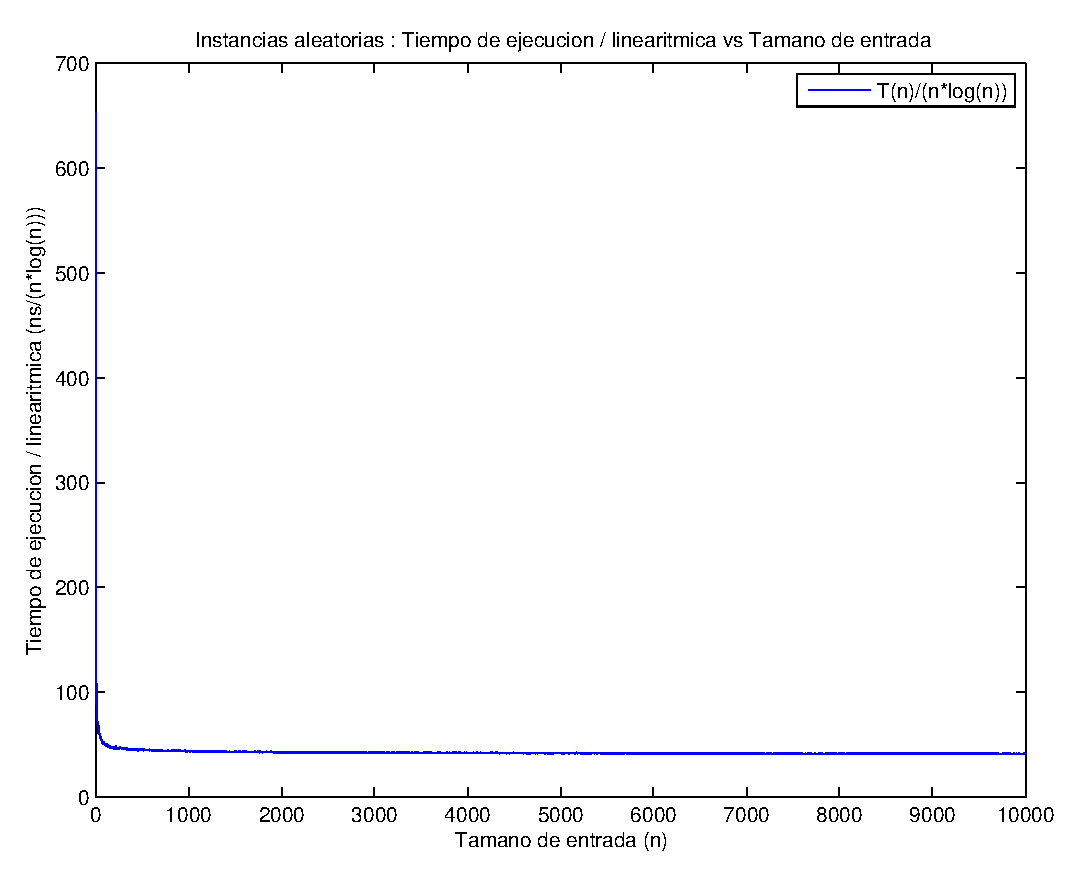
\includegraphics[width=0.5\linewidth]{problema2/graficos/problema2_aleatoria_10000_div_nlogn.eps}
    \caption{Instancias aleatorias, $1 \leq n \leq 10000$. Izquierda: $T(n)$ vs $n$. Derecha: $T(n) / (n * log(n))$ vs $n$.}
    \label{fig:problema2-aleatoria-10000}
  \end{figure}
\end{center}

Además de presentar los datos según fueron medidos, incluimos un gráfico donde se muestra el comportamiento del costo temporal para instancias de tamaño $n$ dividido $n * log(n)$. Esto permite visualizar la tendencia asintótica del cociente $T(n) / (n * log(n))$, que en este caso se aproxima a una constante cercana al valor $50$, sugiriendo dentro del marco de mediciones que $T(n)$ tiende a un crecimiento del orden de $n * log(n)$ para instancias promedio. Esto coincide con el comportamiento observado durante la experimentación del problema \emph{Camiones Sospechosos}, lo cual es de esperarse dado que en ambos casos se utilizó la misma función de ordenamiento para la implementación (ver apéndices \ref{problema1-codigo} y \ref{problema2-codigo}).

\subsubsection{Mediciones sobre el ciclo en instancias ordenadas}

En la figura (\ref{fig:problema2-ciclo}) se muestran los resultados de las mediciones sobre instancias ordenadas, omitiendo el ordenamiento.

\begin{center}
  \begin{figure}[H]
    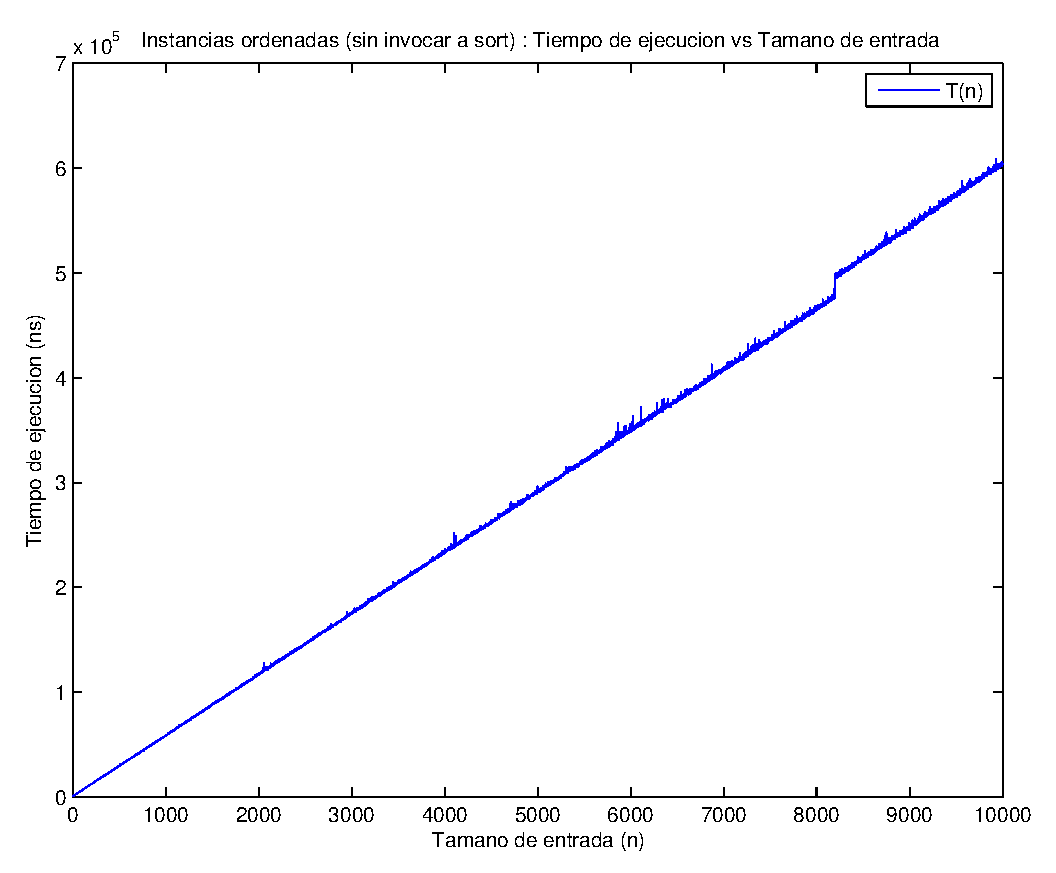
\includegraphics[width=0.5\linewidth]{problema2/graficos/problema2_ordenada_10000.eps}
    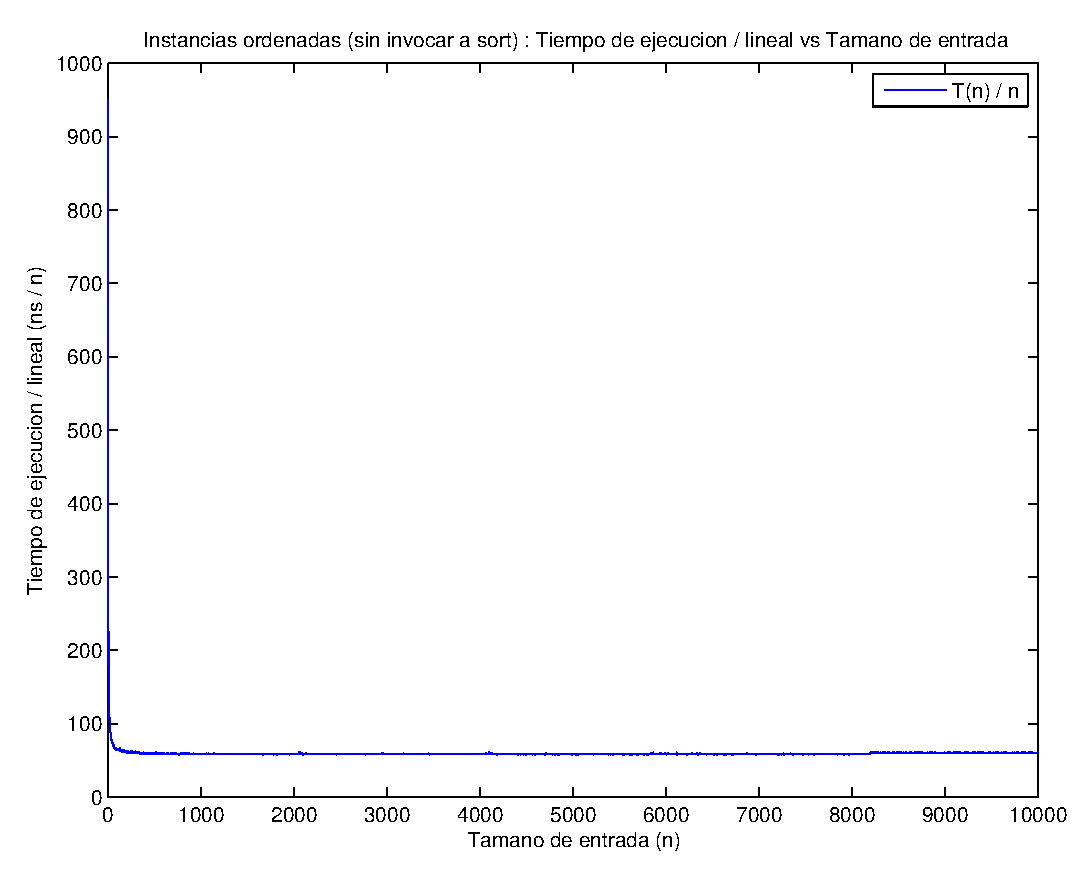
\includegraphics[width=0.5\linewidth]{problema2/graficos/problema2_ordenada_10000_div_n.eps}
  \caption{Instancias aleatorias. $1 \leq n \leq 10000$.}
  \label{fig:problema2-ciclo}
  \end{figure}
\end{center}

Observamos en la curva de costo temporal un crecimiento de orden lineal, con una marcada discontinuidad para $n$ cercano a $8000$. A la vez, incluimos un gráfico mostrando la curva $T(n) / n$ vs $n$\footnote{$T(n)$ en este caso hace referencia a el costo sin la etapa de ordenamiento.}, reiterando sobre la misma técnica utilizada en la sección \ref{problema1-experimentacion}, observando una tendencia hacia un valor constante de aproximadamente $80$ para magnitudes crecientes de $n$. En base a ambas visualizaciones, deducimos que la etapa post-ordenamiento es efectivamente $O(n)$, dado que para la misma no existe distinción entre mejor y peor caso, o caso promedio. Como además es necesario evaluar cada elemento por lo menos una vez al calcular las pérdidas, la etapa es en particular $\Theta(n)$.

Si bien la discontinuidad encontrada no se condice con un comportamiento lineal, aducimos que la misma se debe a cuestiones concretas del contexto de experimentación; por ejemplo, posiblemente debido al tamaño de la memoria caché dado que la posición de la discontinuidad varía cuando realizamos mediciones en equipos de diferentes características.

%Por otro lado, como utilizamos el \emph{sort} de la \emph{stl}, no podemos asegurar si un caso en particular va a ser un ``mejor caso'', o un ``peor caso''. Esto se debe a que, como explicamos anteriormente, el sorting utiliza un \emph{IntroSort} que usa primordialmente un algoritmo similar a \emph{QuickSort}. Por esto al depender del azar, no se puede saber \emph{a priori} si un caso va a ser un ``mejor caso'', o un ``peor caso''.

%Por estas razones, para el ejercicio 2 no incluimos gráficos extra en los cuales hablamos de ``peor caso'' y ``mejor caso''..